% !TeX spellcheck = en

\chapter{Evaluation}
\label{sec:eval}
Chapter describes the evaluation metrics and performed experiments, visualises prediction results.

\section{Goal of evaluation}
\label{sec:eval:goal}
The goal of model evaluation is am estimation of the generalization accuracy of a model on future unseen data. This master thesis aims to evaluate whether RNN neural networks modification as LSTM, GRU and bidirectional variant are able to reduce the positional and rotation error for given look ahead time of 100 ms. This LAT is higher than normal acceptable latency in VR application and even higher that measured M2P latency in cloud streaming platform presented in work \cite{serhan_cloud_streaming}. Since the successfully trained best evaluated model is intended to be build in the server infrastructure, the goal of evaluation is to find out how using of RNN model can reduce the positional and rotational error and thus improve the quality of delivered from cloud server VV content by calculating the proper future 2D image from volumetric data.  

To evaluate all described above models, a Python-based application used for training and processing of the recorded via HoloLens 6-DoF datasets. Below, first Baseline model, the experimental setup and the evaluation metrics are discussed, before presenting the obtained results and discussing the limitations of evaluated models.

\section{Evaluation metrics}
\label{sec:eval:metrics}
Evaluation metrics are used to measure the quality of the predictions made by machine learning model. This thesis similar to work \cite{serhan_kalman} uses two of the most common metrics Mean Absolute Error ($MAE$) and root mean squared error ($RMSE$).

Mean Absolute Error ($MAE$): MAE measures the average error over the test sample of the absolute differences between prediction and actual observation without considering their direction. 
\begin{equation}
MAE= \frac{1}{n} \sum_{j=1}^{n} |y_j - y_{mean}|
\end{equation}

Root mean squared error ($RMSE$): RMSE measures the average magnitude of the error with square root of the average of squared differences between prediction and actual observation.

\begin{equation}
RMSE= \sqrt{ \frac{1}{n} \sum_{j=1}^{n} (y_j - y_{mean})^2}
\end{equation}
Both MAE and RMSE express average model prediction error in units of the variable of interest, both metrics can range from $0$ to $\inf$ and are indifferent to the direction of errors. They are negatively-oriented scores, which means lower values are better\footnote{https://medium.com/human-in-a-machine-world/mae-and-rmse-which-metric-is-better}. Since the errors in $RMSE$ are squared before they are averaged, the RMSE gives a relatively high weight to large errors. Normally, The $RMSE$ result will always be larger or equal to the $MAE$. 

For calculation the metrics for positional data the Euclidean distance (L2 norm) is used.  Rotational metrics calculated with a distance between quaternions represented as an angle between their 3D orientations using a formula:
\begin{equation}
angularDistance = 2*arccos(real(p*conj(q)))
\end{equation}
where $p$ and $q$ are unit quaternions representing two rotations in the same basis and $q*$ denote the quaternion conjugate.

\section{Baseline model}
\label{sec:eval:baseline}
To understand, how actually good evaluated model predicts and helps to reduce the M2P latency, some essentially a simple model that acts as a reference in a machine learning project must be implemented first. Baseline model can lack complexity and may have little predictive power. The LSTM and GRU model should predict much better than a Baseline model and thus comparing the metrics it can be understood how reasonable is the implementing and using of chosen approach. It is intended to use a Baseline model as benchmarks for trained models. There is no rule for what is good or bad model's prediction. The criteria of model evaluation depends on the dataset and use case. A mean square error gives a values in units of the original dataset. For example, if model predicts the prices of apartments in Berlin, then MAE of 1000 is a very good result and market's players would desire to have a trained model to work on the real estate market. However, it is abysmal for a model that predicts the price of average lunch in Berlin's restaurant. Thus a simple predictor is needed to predict a future data so that a predicted values can be compared with the real values using same evaluation metrics as is used for RNN models.

The Baseline in this thesis is similar to the reference model used in the work \cite{serhan_kalman} and represents the operation of the system without prediction. It is assumed that the prediction time is set equal to the M2P latency of 100 ms such that the prediction completely eliminates the latency. Implemented Baseline is a deterministic model, meaning that it produces an expected output given the same input. For LAT of 100 ms a prediction time N is equal to 20 samples. The position and rotation data $x_t$ is simply propagated N samples ahead in the Baseline prediction and set as the user position and rotation at time $x_t + N$, i.e. $Baseline(x_t) = x_{t+N}$. 
\begin{figure}[htb]
	\begin{center}
		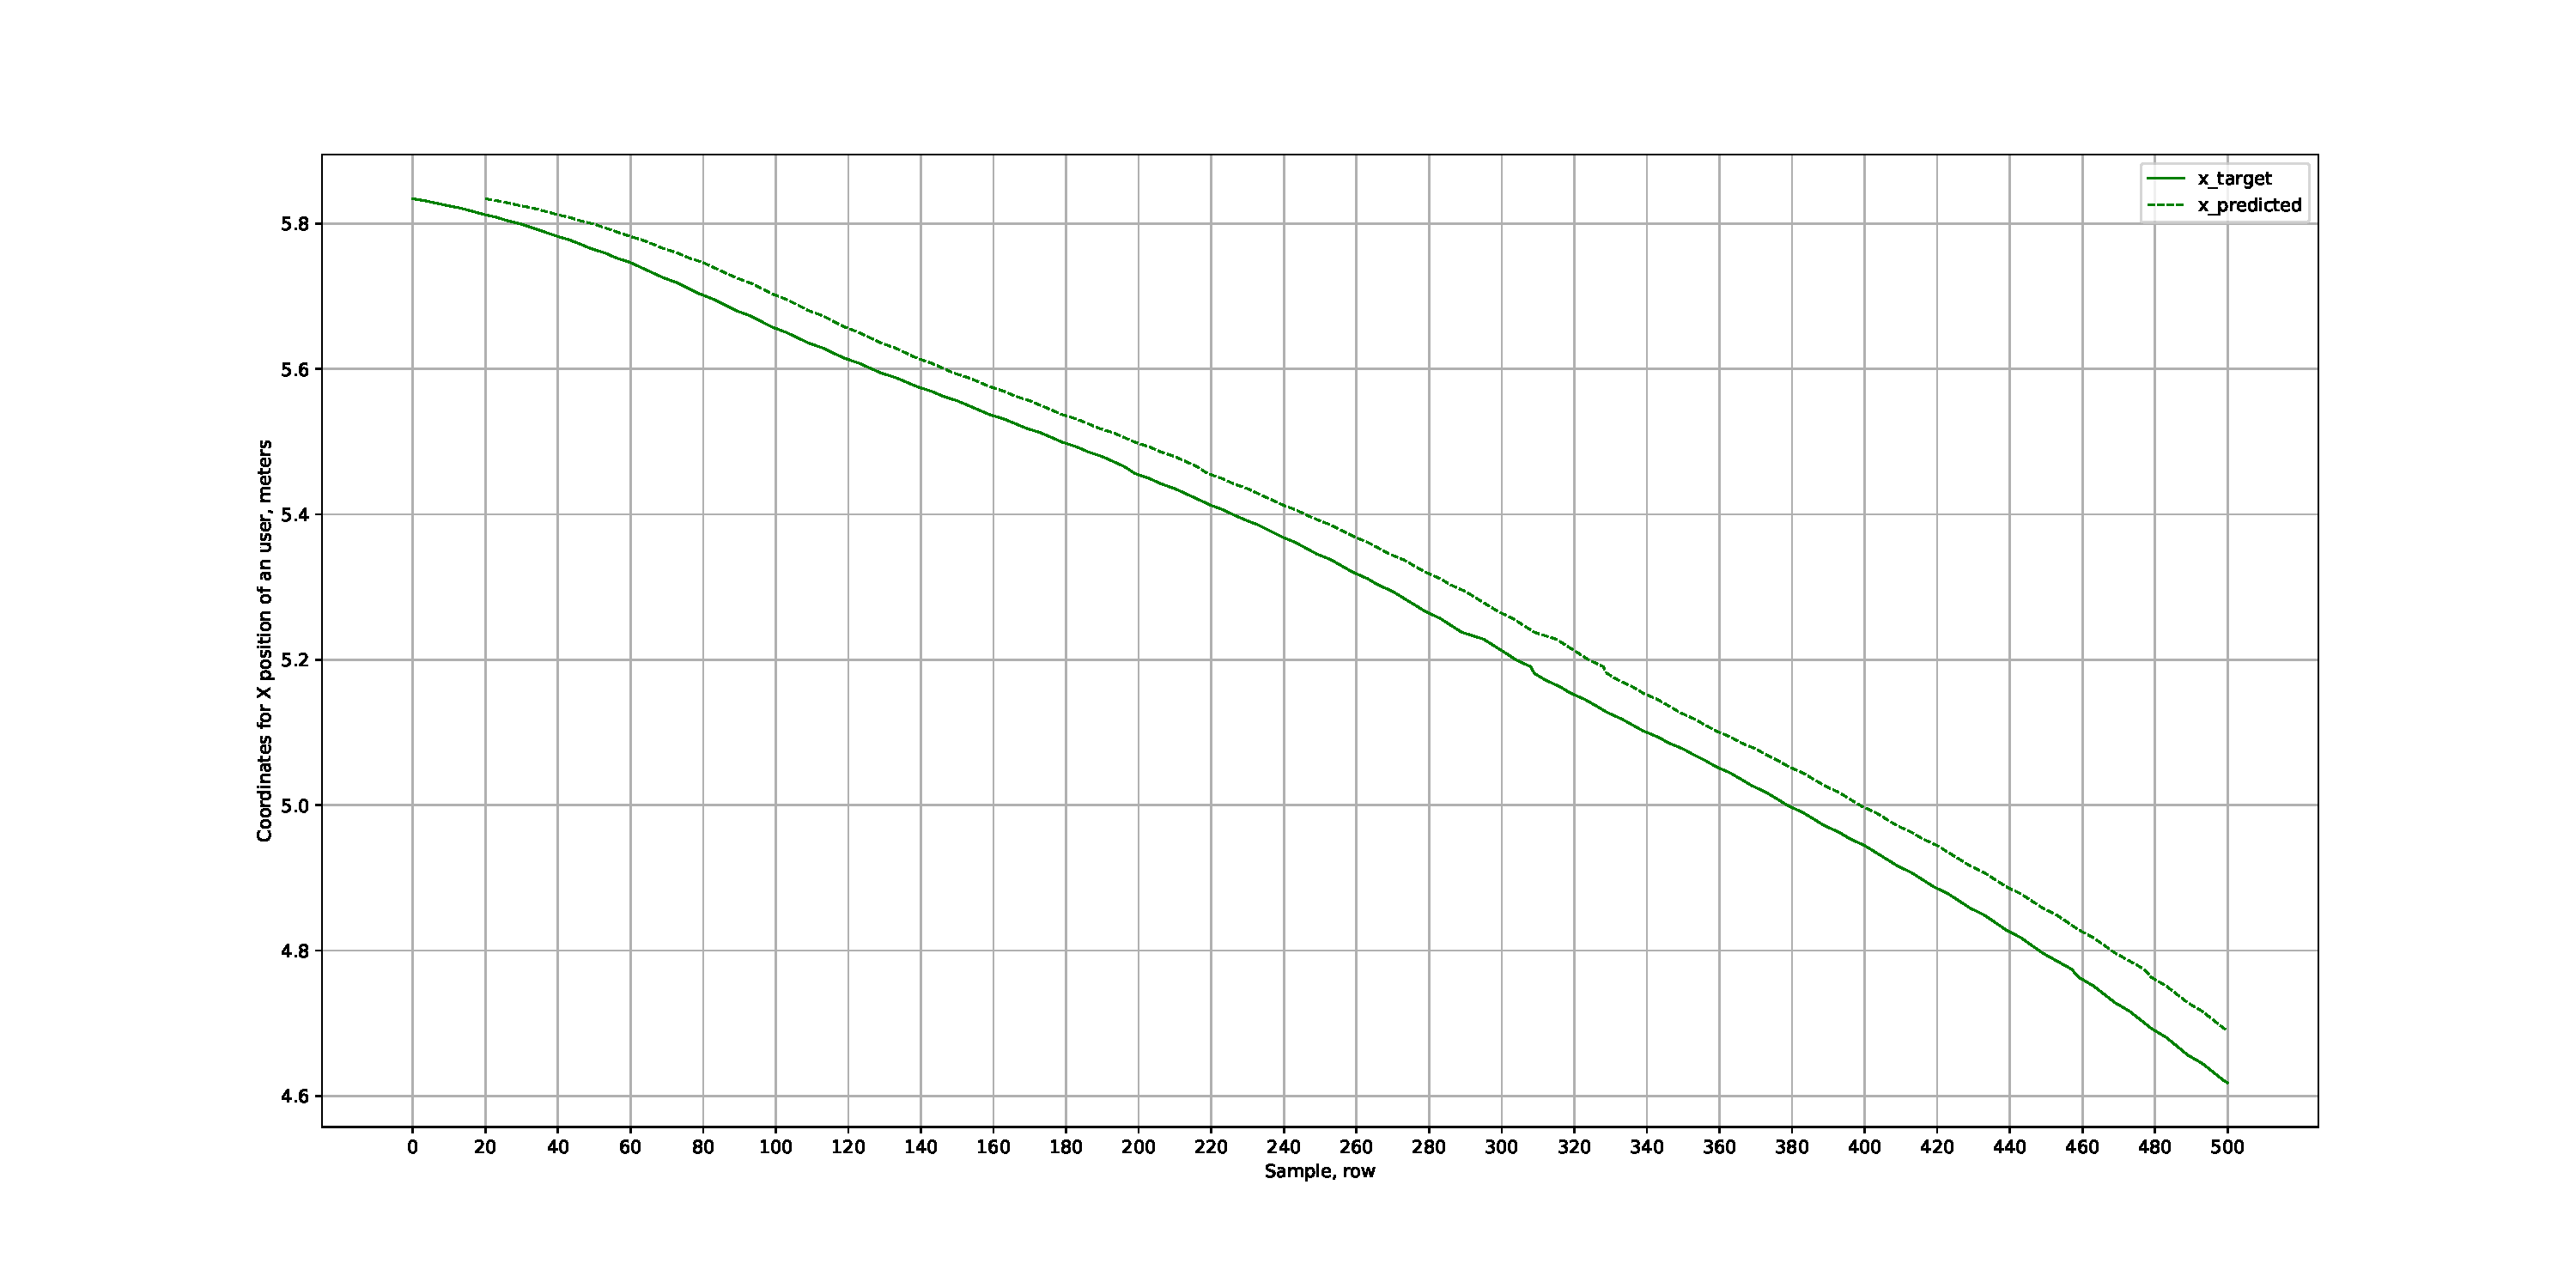
\includegraphics[width=1\textwidth, keepaspectratio]{gfx/base_zoom-x.pdf}
		\caption{\label{fig:base_x} Outputs of Baseline Model for x-axis.}
	\end{center}
\end{figure}

The Fig. \ref{fig:base_x} shows the first 500 real values and the corresponding output of the baseline for positional axis $x$. From the plot of the Baseline model outputs, it is clear that the model is 20-step behind reality. It copies with a given delay the falling trend and all fluctuations of the given axis.

The Fig. \ref{fig:base_xyz} shows the 500 real values and the corresponding output of the baseline for all three positional axes $x, y, z$. The plot samples 500 elements starting from the 2500 row and thus no missing data is seen on Baseline output for the first 20 elements as it plotted in Fig. \ref{fig:base_x}. However, the Fig. \ref{fig:base_xyz} highlights the limitations of the usage of naive predictor that will deliver 2D image created from volumetric video content with a delay of 100 ms that is unappropriated delay for a human to experience in VR application without physical consequences like motion sickness \cite{delay_sickness}. The mean square error for the all three positional axes $MAE = 0.067$m and root mean square error  $RMSE = 0.068$m meaning the average distance between predicted position and the real position is equal to almost 7 cm. It is not crucial when an user looks on the big VV object, like a volumetric humans hologram, from the distance of 3-4 meters. But if an user interacts with the small VV objects presented in the VR environment, then this distance became a significant difference between what user will see with a delay and where the VR object would be placed for delayed position. 

\begin{figure}[htb]
	\begin{center}
		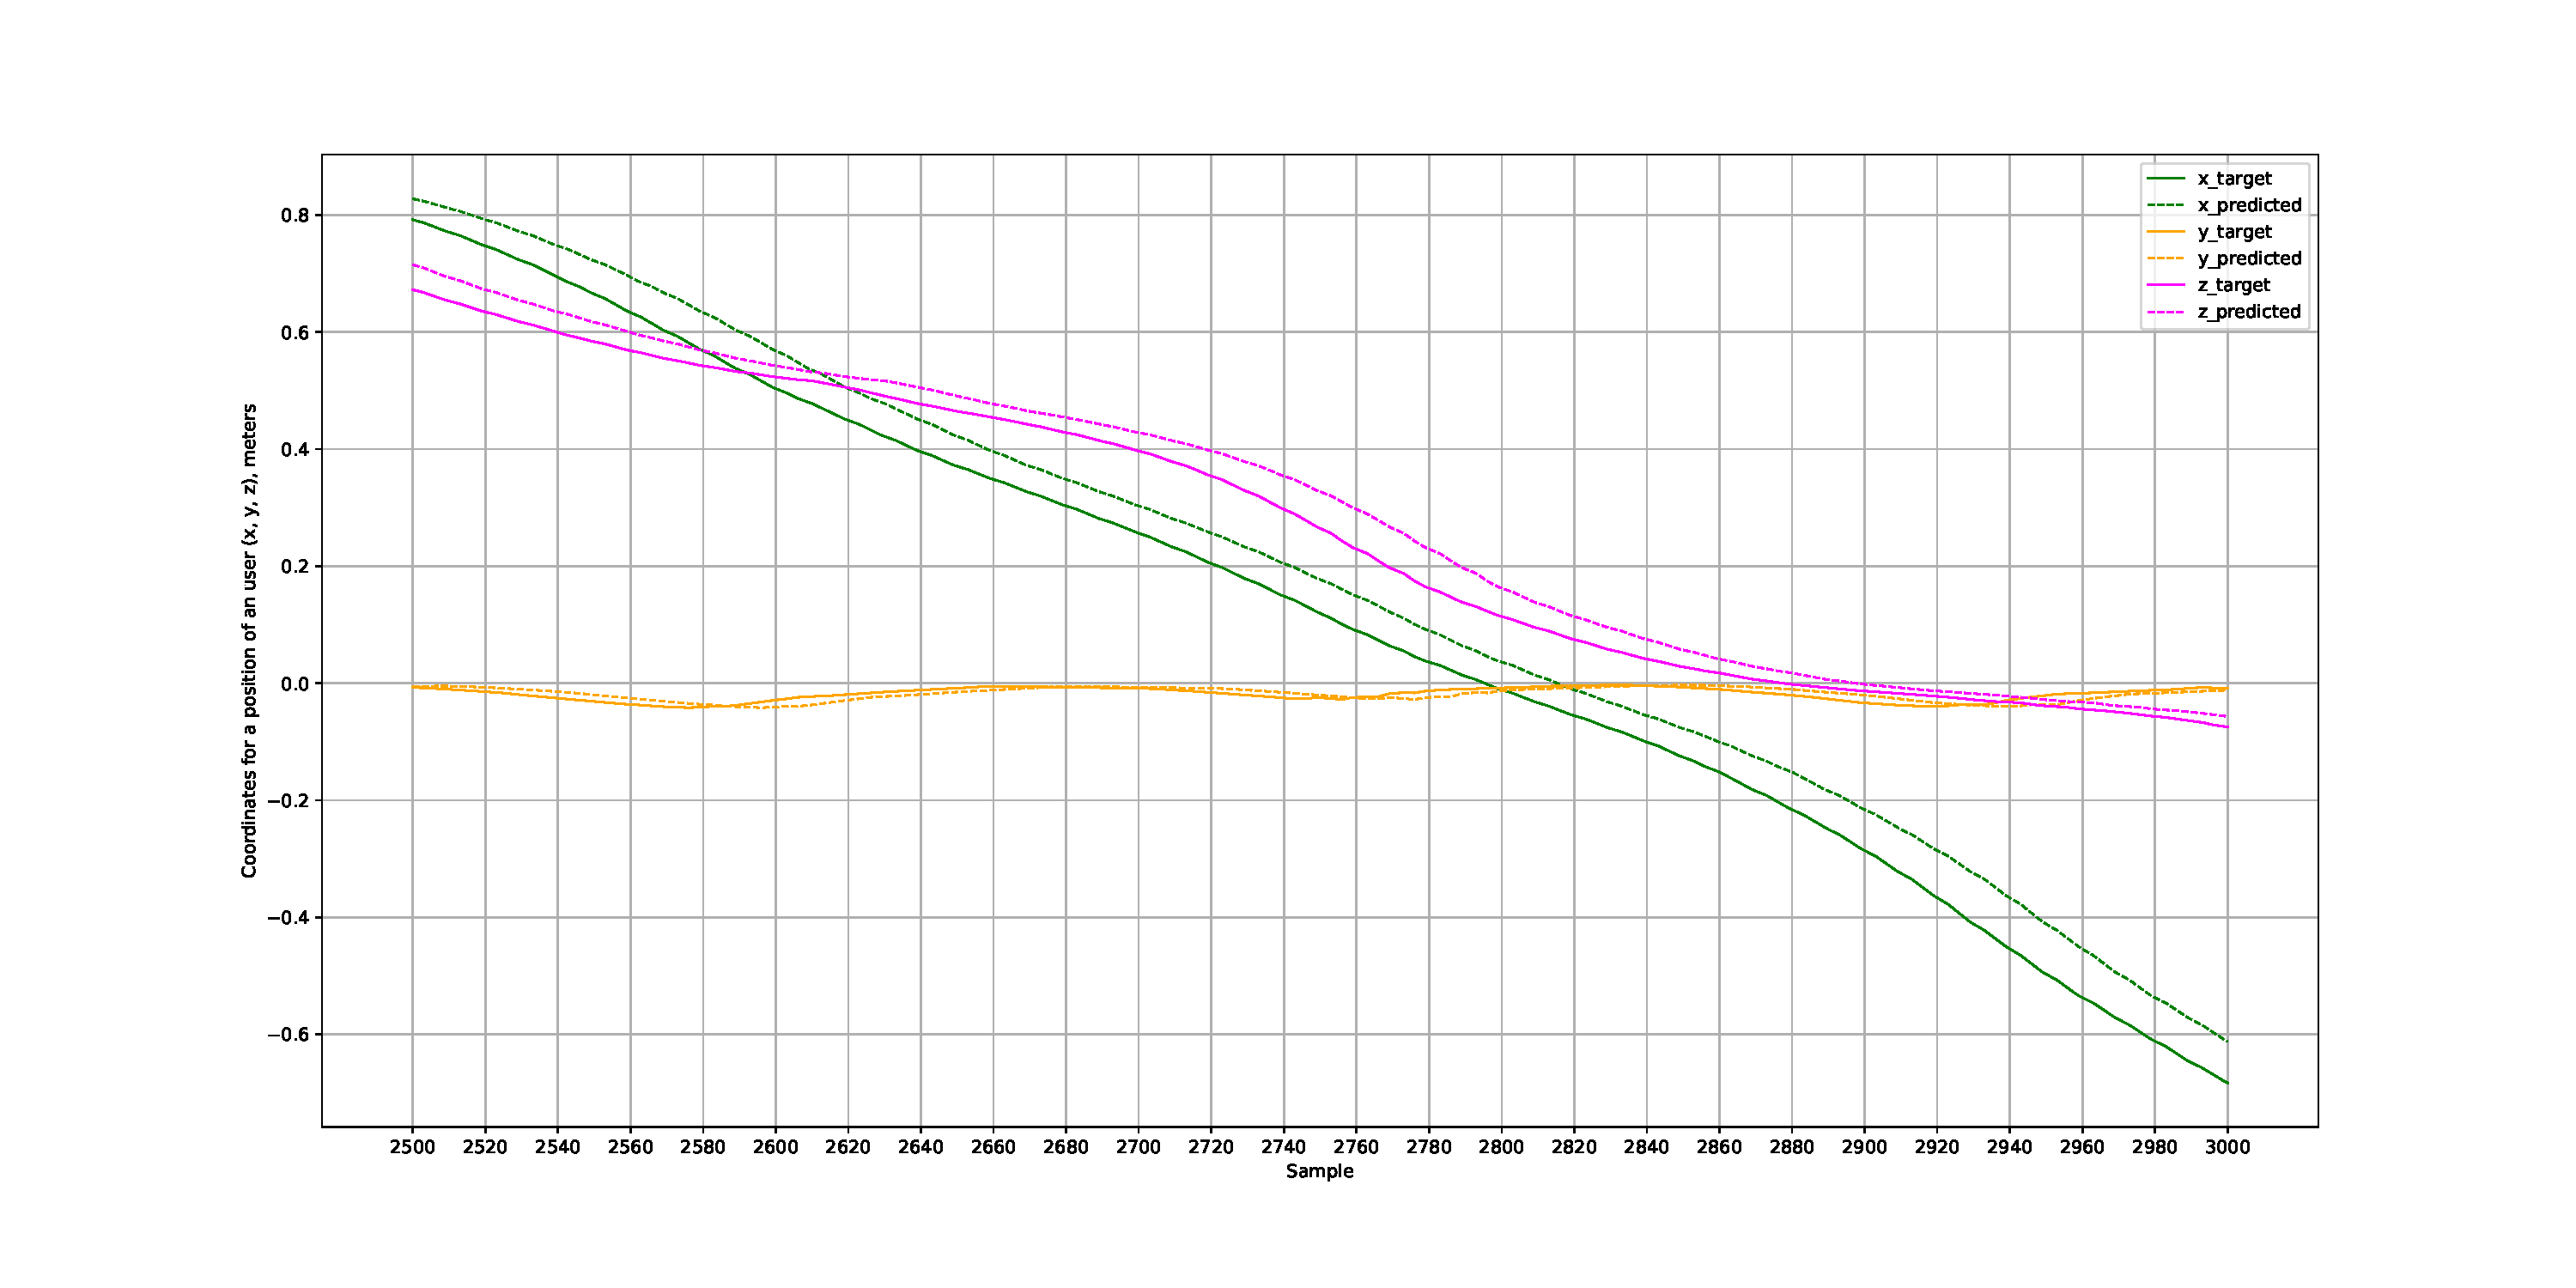
\includegraphics[width=1\textwidth, keepaspectratio]{gfx/base_zoom-xyz_position.pdf}
		\caption{\label{fig:base_xyz} Outputs of Baseline Model for x, y and z axes.}
	\end{center}
\end{figure}

It is worth to mention that in the case if real data is neither increasing nor decreasing in the given interval and fluctuates near the constant value, as it seen at $y$-axis, than the delay of the Baseline output is more not obvious when visualized due the overlapping of two graphs. In fact, the Baseline outputs have the same delay as those one with good visualized delay as, for example, $x$-axis.

Fig. \ref{fig:base_quat_xyzw} shows the Baseline outputs for quaternions components $qx, qy, qz$ and $qw$. Same as with positional data, the same delay of 20 samples is present on rotational data. For all four quaternion components calculated metrics  are: $MAE = 3.12^{\circ}$ and $RMSE =3.24^{\circ}$ .  

\begin{figure}[htb]
	\begin{center}
		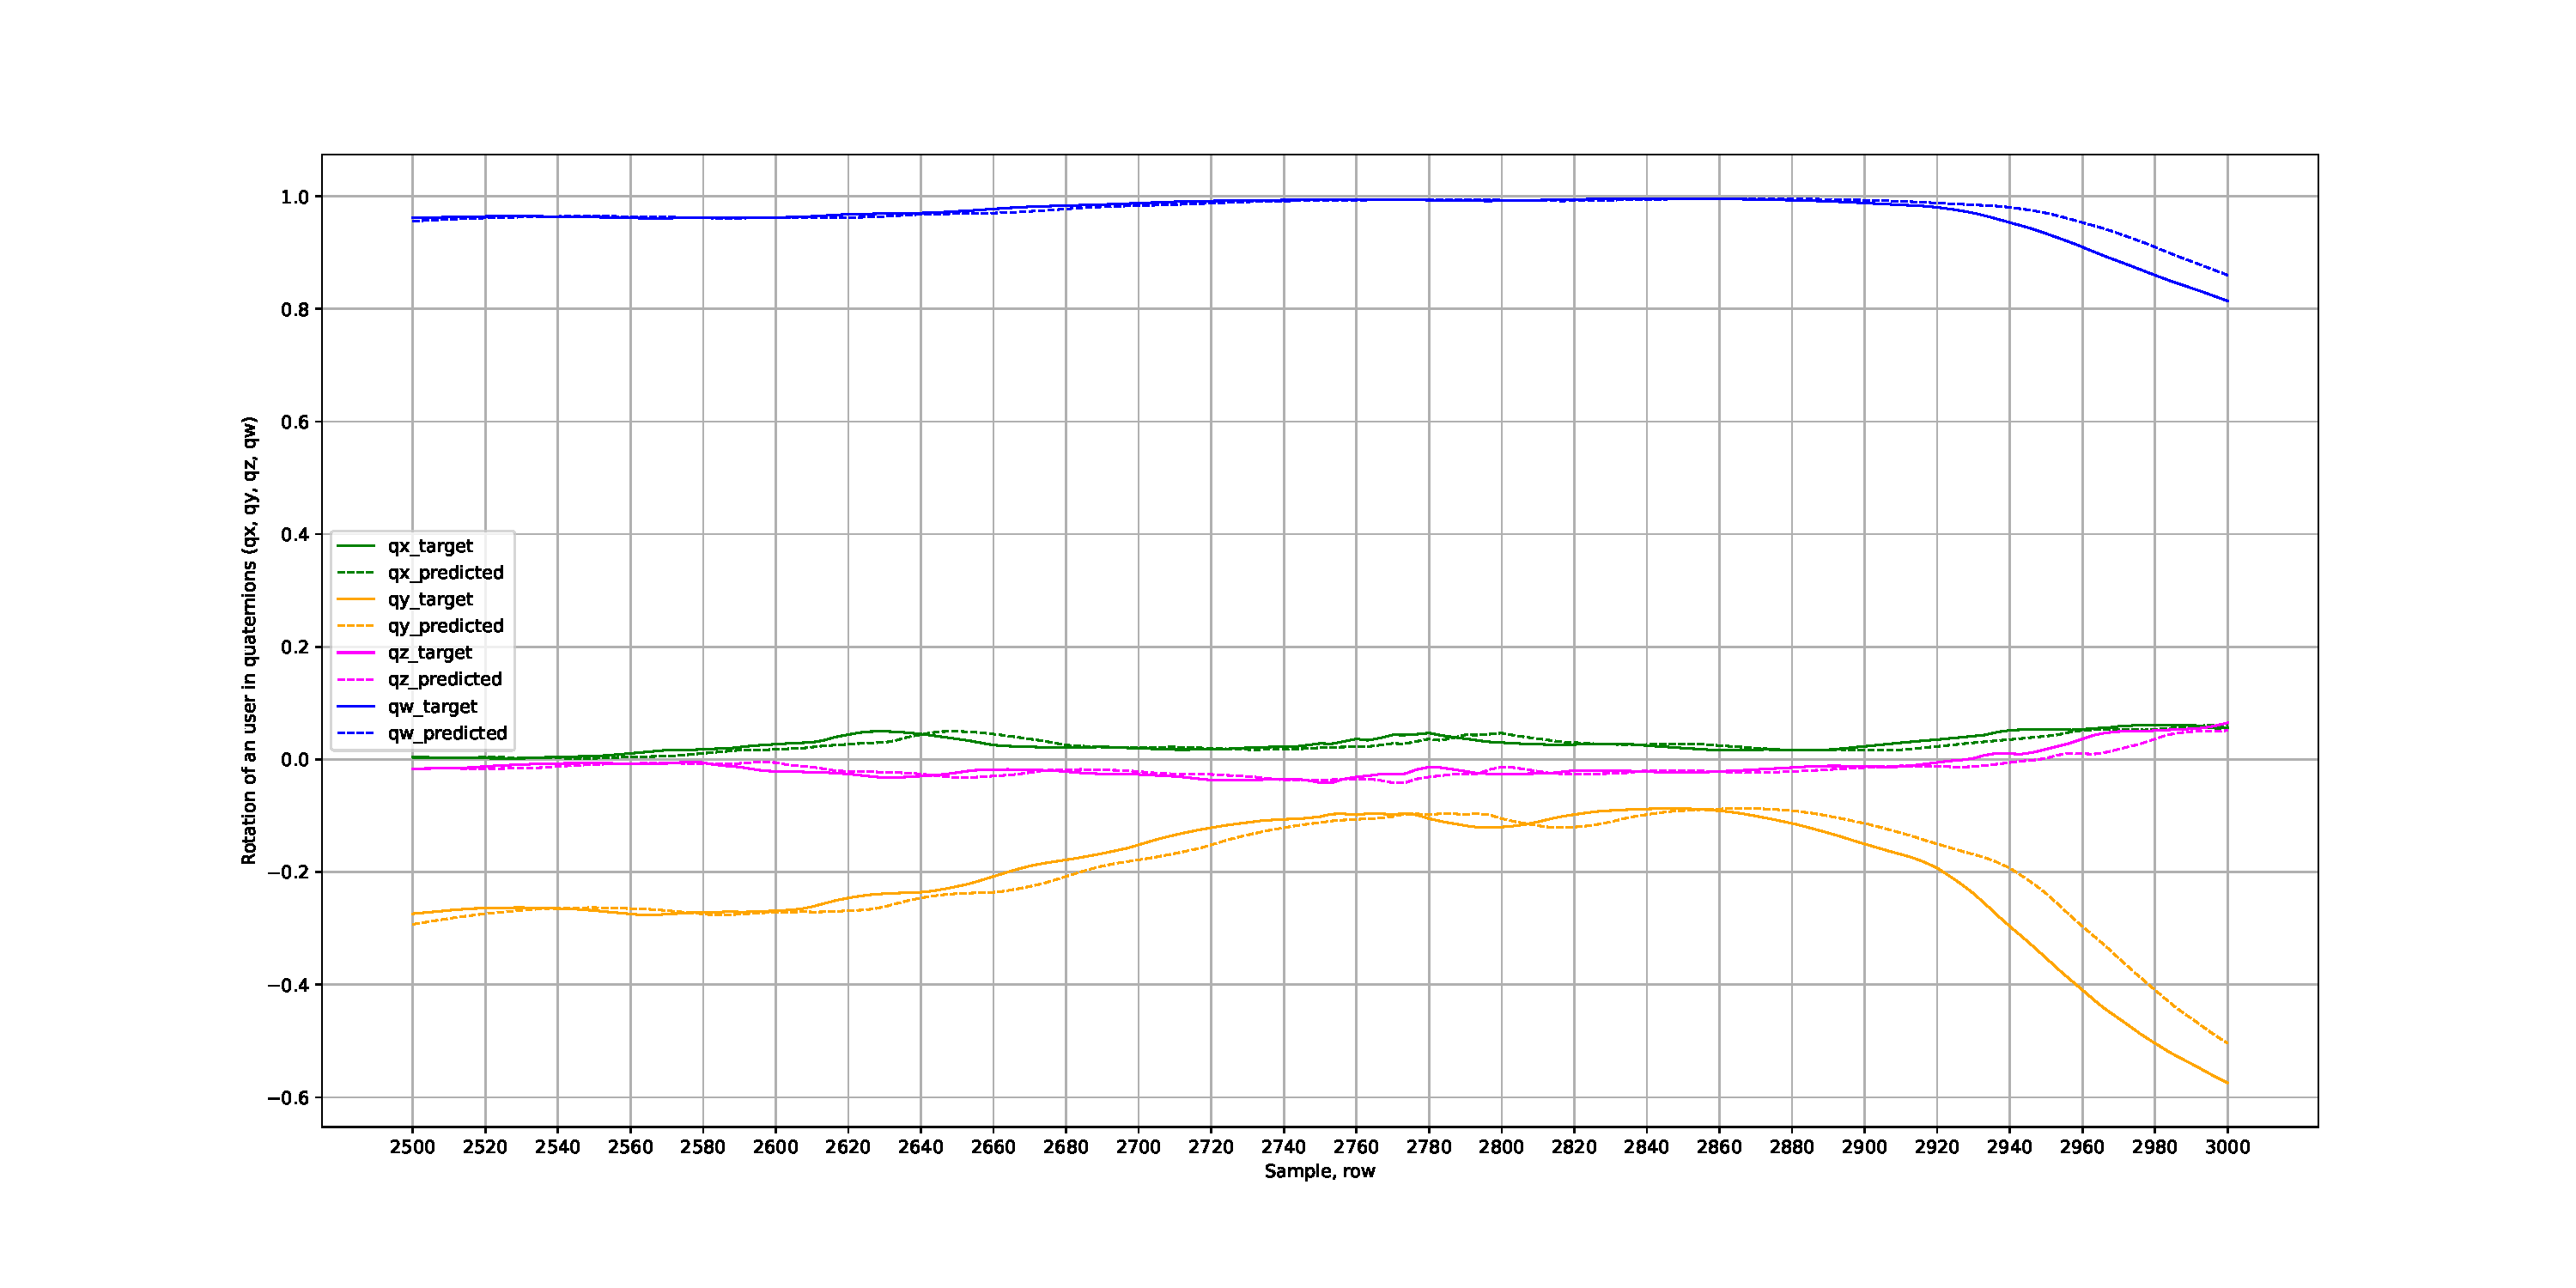
\includegraphics[width=1\textwidth, keepaspectratio]{gfx/base_zoom-qx_qy_qz_qw_rotation.pdf}
		\caption{\label{fig:base_quat_xyzw} Outputs of Baseline Model for quaternions components qx, qy. qz and qw.}
	\end{center}
\end{figure}

Because metrics of rotational data is measured in degrees, for visualization purposes, orientations are given in the Fig. \ref{fig:base_euler} as Euler angles (yaw, pitch, roll), although prediction is performed in the quaternion domain.

\begin{figure}[htb]
	\begin{center}
		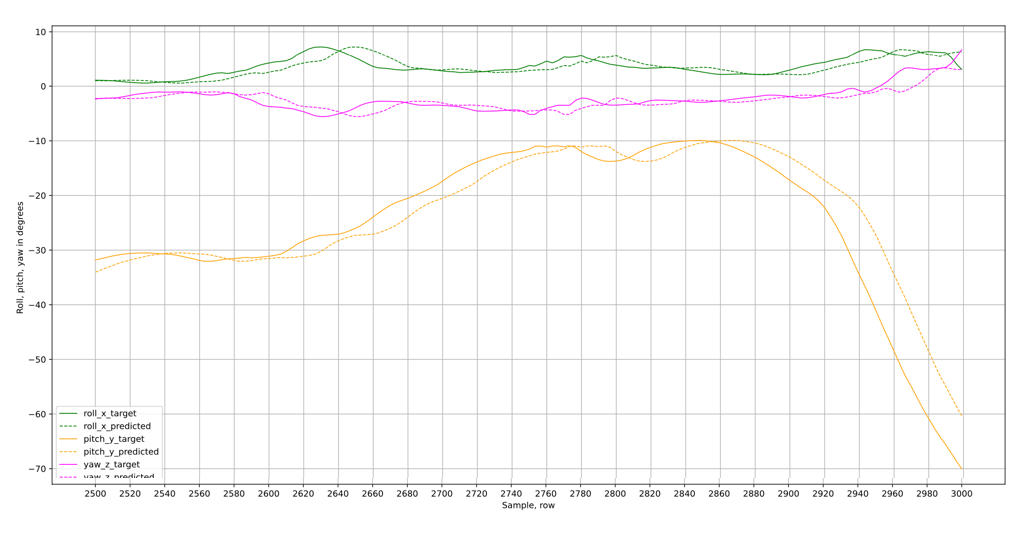
\includegraphics[width=0.85\textwidth, keepaspectratio]{gfx/base_euler-roll_pitch_yaw.png}
		\caption{\label{fig:base_euler} Outputs of Baseline Model for rotation data represented as Euler angles.}
	\end{center}
\end{figure}

The evaluated RNN model is considered to be successfully trained if the $MAE$ and $RMSE$ metrics at least for positional or rotational data can show significant improvement comparing to a Baseline output. 

\newpage
\section{Experiments}
\label{sec:eval:experiments}
In the experiments implemented models were trained with different hyperparameters and evaluated using $MSE$ and $RMSE$ metrics. 

\subsection{First experiments}
\label{sec:eval:experiments:early}

\subsubsection{Datasets}
\label{sec:eval:experiments:early:ds}
As already stated in section \ref{sec:design:dataset:preprocessing}

\subsubsection{Batch size}
\label{sec:eval:experiments:early:batch}
A significant impact on the performance e.g. the prediction accuracy has a batch size used in LSTM or GRU models. The batch-size helps to learn the common patterns as important features by providing a fixed number of samples at one time. So that the model thus can distinguish the common features by looking at all the introduced samples of the batch. In most cases, an optimal batch size is set to 64. When this batch size was initially used with LSTM model, it gave significant high MSE, RMSE, train and validation errors. Based on the performance observation during experiments with LSTM parameters, batch size fine-tuning was done. The experiments done by \textit{Aykut et al} in their works \cite{delay_compensation_360} and \cite{telepresence} proved that appropriate batch size can be found in range $2^{9}$ - $2^{11}$ (512 - 2048). Notice that a power of 2 is used as a batch size. The overall idea is to fit a batch of samples entirely in the the CPU/GPU. Since, all the CPU/GPU comes with a storage capacity in power of two, it is advised to keep a batch size a power of two. Using a number different from a power of 2 could lead to poor performance. Experimentally is proved in this thesis that similar to works \cite{delay_compensation_360, telepresence}  batch size of $2^{8}$ - $2^{10}$ (256, 512 and sometimes 1024) produces the best prediction result on 6-DoF dataset if the other hyperparameters are set correctly. The smaller batch sizes (32, 64 and 128) resulted in the high values of evaluation metrics and it was obvious to notice during experiments the improving the metrics with increasing the batch size.

\subsubsection{Learning rate}
\label{sec:eval:experiments:early:lr}
Learning rate is a parameter of extended version of stochastic gradient Adam optimizer. The learning rate determines how much an updating step influences the current value of the weights. Adam optimizer has an additional term in the weight update rule that causes the weights to exponentially decay to zero, if no other update is scheduled.

If learning rate is large then a correspondingly large modification of the weights $w_i$ happens on each epoch. In general too large learning rate overshoots the local minimum in a cost function.

\subsection{Prediction with LSTM}
\label{sec:eval:experiments:lstm}
!!!
During preprocessing step Euler angles (yaw, pitch, roll) were calculated from quaternions and these parameters are used for visualization purposes. Although the interpolated $csv$-file contains additional Euler angles columns, only described in section \ref{sec:design:dataset:HL} parameters were used for training and prediction.
%%%%%%#
!!!!!



\subsection{Prediction with GRU}
\label{sec:eval:experiments:gru}

\subsection{Prediction with Bidirectional GRU}
\label{sec:eval:experiments:bi-gru}